\documentclass{article}

% Language setting
% Replace `english' with e.g. `spanish' to change the document language
\usepackage[french]{babel}
\usepackage[T1]{fontenc}

% Set page size and margins
% Replace `letterpaper' with `a4paper' for UK/EU standard size
\usepackage[a4paper,top=2cm,bottom=2cm,left=3cm,right=3cm,marginparwidth=1.75cm]{geometry}

% Useful packages
\usepackage{amsmath}
\usepackage{graphicx}
\usepackage[colorlinks=true, allcolors=blue]{hyperref}
\usepackage{minted}
\usepackage{forest}
\usepackage{caption}

\title{Projet en informatique pour les sciences humaines}
\author{Johan Cuda}

\begin{document}
\maketitle

\begin{abstract}
Ce projet reprend le travail de \textit{threading} des widgets de Orange Textable effectué par Antonin Schnyder en proposant de remonter l'architecture de \textit{threading} d'un étage dans la hiérarchie de classes de Textable. 
\end{abstract}

\tableofcontents

\section{Introduction}

\subsection{Contexte}

\href{http://textable.io/}{Textable} est un add-on du logiciel \href{https://orangedatamining.com/}{Orange} qui permet d'analyser des textes de manière visuelle \footnote{Xanthos, Aris (2014). Textable: programmation visuelle pour l’analyse de données textuelles. In Actes des 12èmes Journées internationales d’analyse statistique des données textuelles (JADT 2014), pp. 691-703. \href{http://lexicometrica.univ-paris3.fr/jadt/jadt2014/01-ACTES/57-JADT2014.pdf}{Read online}}; il est composé de widgets développés en Python qui ont récemment été modifiés par Antonin Schnyder pour optimiser leur processus. En effet, l'interface des widgets se bloquant pendant les traitements de données et leurs performances pouvant être optimisées, Antonin Schnyder a modifié ces widgets pour ajouter une logique de \textit{threading} \footnote{À ce sujet voir \href{https://realpython.com/intro-to-python-threading/}{An Intro to Threading in Python}.} qui suit les recommandations de Orange \footnote{Le tutoriel de Orange à ce propos est disponible \href{https://orange3.readthedocs.io/projects/orange-development/en/latest/tutorial-responsive-gui.html}{ici}.}.\newline

Dans ce travail, nous proposons de partir du travail effectué par Antonin Schnyder en remontant d'un étage – dans la hiérarchie de classes de Textable – la logique de \textit{threading}. Nous avons identifié qu'une grande partie du code qui permet la mise en place du \textit{threading} se répète dans les widgets, nous avons donc modifié  leur architecture pour faire en sorte que les éléments liés au \textit{threading} soient hérités au travers de la super-classe \textbf{OWTextableBaseWidget}.
\newline

Nous commencerons par discuter rapidement de ce qu'est le \textit{threading}, puis par expliciter la structure du add-on \textit{Textable} ainsi que d'un widget typique pour mieux comprendre leur fonctionnement. Ensuite, nous listerons les éléments que nous avons identifiés comme possiblement remontables, en mentionnant ceux qui ont directement pu être remonter et en décrivant les modifications effectuées sur ceux qui ne le pouvaient pas. Ce faisant, nous discuterons des divers problèmes rencontrés pendant l'implémentation. Nous termienrons ce rapport en proposant un tutoriel de développement de widget qui permet d'exploiter cette nouvelle architecture ainsi que d'assurer en partie l'uniformité des futures widgets qui seront ajoutés à \textit{Textable}. Ce tutoriel reprendra en partie le \href{https://docs.google.com/document/d/1QtXm2aYMZXAyM7mfBTqxt_XrTNFqC7e3aqy7OC1A_18/edit}{tutoriel fourni par Antonin Schnyder}.

\subsection{Qu'est-ce que le \textit{threading}?}

Ce projet n'a pas pour but d'expliquer ce qu'est le \textit{threading} mais il est quand même nécessaire de fournir une explication succincte du concept pour mieux appréhender le travail proposé dans ce rapport.
Le \textit{threading} répartit le travail entre différents \textit{threads} et de simule une forme de \textit{multiprocessing}\footnote{Sur la différence entre m\textit{multiprocessing} et \textit{multithreading} voir \href{https://www.geeksforgeeks.org/difference-between-multithreading-vs-multiprocessing-in-python/}{ce lien}.}. À la création de chaque widget, un \textit{main thread} est créé et s'occupera de différents \textit{worker threads} qui seront créés par chaque widget. Le \textit{multithreading} consiste ensuite à faire s'enchaîner l'exécution des \textit{worker threads} pour simuler une sorte de parallélisme des processus. Dans le cas particulier de \textit{Textable}, les processus qui sont voués à être exécutés dans un \textit{worker thread} sont les appels aux fonctions de \href{https://github.com/axanthos/LTTL}{LTTL} par exemple.
Ce système permet donc d'améliorer les performances d'un \textit{software} mais aussi dans notre cas précis de permettre à l'\textit{User interface} (UI) de notre widget de ne pas se bloquer pendant ses calculs. Ceci est extrêmement utile en considérant que suivant la taille des corpus analysés avec \textit{Textable}, les calculs peuvent prendre du temps, il est donc pratique de pouvoir annuler le processus en cours grâce au bouton \texttt{Cancel} par exemple.

\section{Structure de \textit{Textable} et des widgets}

\subsection{Structure de \texttt{TextableUtils.py} et \textbf{OWTextableBaseWidget}}

\textit{Textable} peut être visulisé de la manière suivante :
\vspace{5mm}


\begin{figure}[h]
    \centering
    \fbox{%
    \begin{forest}
    for tree={
        font=\ttfamily,
        grow'=0,
        child anchor=west,
        parent anchor=south,
        anchor=west,
        calign=first,
        edge path={
            \noexpand\path [draw, \forestoption{edge}]
            (!u.south west) +(5pt,0) |- (.child anchor)\forestoption{edge label};
        },
        inner sep=1pt,
        l=1cm,
        s sep=2mm,
        edge+={darkgray, line width=0.5pt},
        if level=0{
            align=center,
        }{%
            if level=1{font=\bfseries}{}% folder level
        },
        fit=band,
        before typesetting nodes={
            if n=1
                {insert before={[,phantom]}}
                {}
        },
        before computing xy={l=15pt},
    }
    [\_textable
        [\_\_init\_\_.py]
        [\_\_pycache\_\_]
        [widgets
            [\_\_init\_\_.py]
            [\_\_pycache\_\_]
            [icons]
            [OWTextableCategory.py]
            [...]
            [TextableUtils.py]
        ]
    ]
    \end{forest}
    }
    \caption{Structure du projet Textable}
    \label{fig:textable_tree}
\end{figure}
\vspace{5mm}

Pour bien comprendre la structure de \textit{Textable}, nous allons commencer par considérer le script \texttt{TextableUtils.py} (voir Figure \ref{fig:textable_utils}). Celui-ci contient plusieurs classes qui définissent des éléments utilisables par tous les widgets comme \texttt{InfoBox} ou \texttt{SendButton}. La classe qui nous intéressera le plus sera bien entendu \textbf{OWTextableBaseWidget} : contenant les éléments de base nécessaires à tous les widgets de \textit{Textable}, elle est déjà héritée par ceux-ci et a donc été rapidement identifiée comme la classe qui recevrait les modifications relatives au \textit{threading}.

\vspace{5mm}

\begin{figure}[htbp]
    \centering
    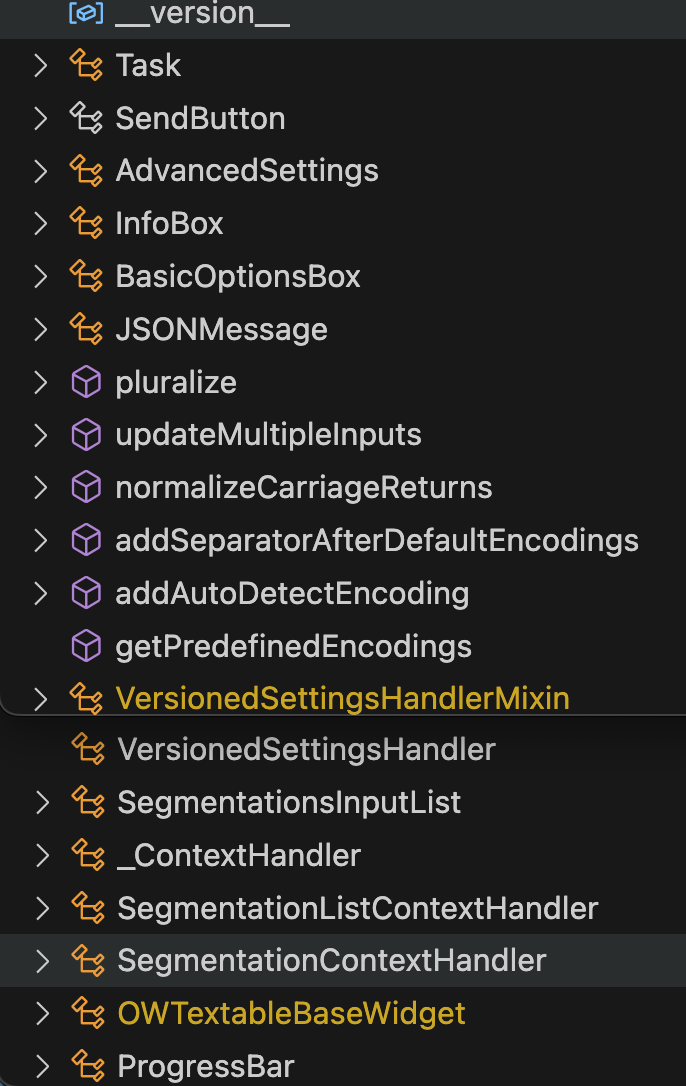
\includegraphics[width=0.25\textwidth]{structure_utils.png}
    \caption{Structure de \texttt{TextableUtils.py}}
    \label{fig:textable_utils}
\end{figure}

\subsection{Structure d'un widget type}

Les widgets ont une structure assez uniforme et représentent chacun une \textit{classe} spécifique qui hérite de la classe \textbf{OWTextableBaseWidget} (par exemple chaque widget \texttt{Count} est une instance de la classe \textbf{OWTextableCount(OWTextableBaseWidget)}). Ils sont toujours formés des éléments suivants : 

\begin{enumerate}
    \item Imports de modules divers
    \item Déclaration d'une série d'\textit{attributs de classes}
    \item Déclaration, dans le constructeur de la classe, de tous les \textit{attributs d'instance} ainsi que des éléments d'interface du widget
    \item Déclaration des diverses méthodes propres au processus du widget
\end{enumerate}

La structure générale peut varier selon les widgets mais nous avons ici les éléments principaux.

\section{Analyse des widgets et implémentation}

Nous avons commencé – sur recommandation d'Aris Xantos – par analyser les deux widgets \texttt{Count} et \texttt{Preprocess}, car ils sont assez représentatifs de deux types de widgets courants dans \textit{Textable}. Nous avons donc systématiquement repéré tous les éléments liés au \textit{threading} dans ces deux widgets pour ensuite évaluer s'ils étaient remontables dans la classe parente \textbf{OWTextableBaseWidget} ou non. Nous avons ensuite étendu notre réflexion aux autres widgets pour finalement trouver des solutions d'implémentation. Dans la suite de cette section, nous adopterons les conventions suivantes : 

\begin{itemize}
    \item \texttt{NomDuWidgetThread} pour nommer la version du widget développée par Antonin Schnyder (par exemple \texttt{ConvertThread} dans le cas du widget \texttt{Convert})
    \item \texttt{NomDuWidgetThreadJohan} pour nommer la version du widget  développée dans le cadre de ce rapport (par exemple \texttt{PreprocessThreadJohan} dans le cas de \texttt{Preprocess})
    \item "\textbf{\# ...}" pour représenter une ellipse dans un extrait de code
    \item "Nous avons donc \textbf{remonté} tel élément..." signifie que nous avons \textit{déplacé} l'élément d'un étage dans la hiérarchie de classes de \textit{Textable}, spécifiquement dans la classe \textbf{OWTextableBaseWidget} de \texttt{TextableUtils.py} 
\end{itemize}

\subsection{Méthodes et attributs remontés mais non-modifiés}

Nous allons ici étudier tous les éléments présents dans les widgets créés par Antonin Schnyder qui ont pu être déplacés dans \texttt{TextableUtils.py} sans modifications particulières. Nous fournirons aussi l'extrait de code déplacé.

\subsubsection{Signaux et slots}

Pour afficher certaines informations sur l'interface (par exemple des messages dans l'\texttt{InfoBox} ou l'avancée de la \texttt{ProgressBar}) pendant le processus d'un widget \textit{threadé}, il est nécessaire de définir des signaux (comme \textit{attributs de classe}) et de les connecter à des slots (qui sont des méthodes qui seront explicitées dans la prochaine section), ce qui permettra aux \textit{worker threads} de communiquer avec l'interface du widget d'une manière \textit{thread safe} (i.e. qui prend en compte l'exécution des \textit{threads} et qui ne tente pas de forcer l'\textit{update} de l'UI). 
\newline

Exemple du code présent dans le widget \texttt{CategoryThread}:


\begin{minted}{python}
    class OWTextableCategory(OWTextableBaseWidget):
        """Orange widget for extracting content or annotation information"""

        # ...

        # Signals
        signal_prog = pyqtSignal((int, bool))       # Progress bar (value, init)
        signal_text = pyqtSignal((str, str))        # Text label (text, infotype)
        signal_cancel_button = pyqtSignal(bool)     # Allow to Deactivate cancel
                                                    # button from worker thread

        # ...
        
        def __init__(self):

            """Initialize a Category widget"""

            # ...

            # Connect signals to slots
            self.signal_prog.connect(self.update_progress_bar) 
            self.signal_text.connect(self.update_infobox)
            self.signal_cancel_button.connect(self.disable_cancel_button)
\end{minted}

Tous les widgets n'ont pas forcément besoin de tous les signaux \footnote{À ce sujet voir le \href{https://docs.google.com/document/d/1QtXm2aYMZXAyM7mfBTqxt_XrTNFqC7e3aqy7OC1A_18/edit}{tutoriel} D'antonin Schnyder.}, nous avons pourtant décidé de remonter les trois signaux comme attributs de la classe \textbf{OWTextableBaseWidget} en partant du principe que de faire hériter les trois signaux à tous les widgets ne crée pas de problème particulier et permet de standardiser le code de tous les widgets. 
\vspace{5mm}

Le résultat dans \texttt{TextableUtils.py} est donc le code suivant : 

\begin{minted}{python}
    class OWTextableBaseWidget(widget.OWWidget):
        """
        A base widget for other concrete orange-textable widgets.
    
        Defines s common `uuid` setting which is required for all Textable
        widgets.
    
        """

        # ...

        # Signals
        signal_prog = pyqtSignal((int, bool))       # Progress bar (value, init)
        signal_text = pyqtSignal((str, str))        # Text label (text, infotype)
        signal_cancel_button = pyqtSignal(bool)     # Allow to Deactivate cancel
                                                    # button from worker thread

        # ...
        
        def __init__(self, *args, **kwargs):

            """Initialize a Category widget"""

            # ...

            # Connect signals to slots
            self.signal_prog.connect(self.update_progress_bar) 
            self.signal_text.connect(self.update_infobox)
            self.signal_cancel_button.connect(self.disable_cancel_button)
\end{minted}

\subsubsection{Méthodes liées aux signaux}

Lorsqu'un signal est émis depuis un \textit{thread} (par exemple pour faire avancer la \texttt{ProgressBar}),  le \textit{slot} – une méthode particulière reliée au signal et décorée par \texttt{@pyqtSlot()} – correspondant est appelé. Dans la version des widgets d'Antonin Schnyder, il était nécessaire de définir autant de slots que de signaux.

\vspace{5mm}
Exemple de slot pour mettre à jour la \texttt{ProgressBar}:

\begin{minted}{python}
    @pyqtSlot(int, bool)
    def update_progress_bar(self, val, init):
        """ Update progress bar in a thread-safe manner """
        # Re-init progress bar, if needed
        if init:
            self.progressBarInit()
        
        # Update progress bar
        if val >= 100:
            self.progressBarFinished() # Finish progress bar     
        elif val < 0:
            self.progressBarSet(0)
        else:
            self.progressBarSet(val)
\end{minted}

Comme dans le cas de signaux, nous avons décidé de remonter les trois slots \texttt{update\_progress\_bar}, \texttt{update\_infobox} et \texttt{disable\_cancel\_button} dans \texttt{TextableUtils.py}, même s'ils ne sont pas tous utilisés par chaque widget. En remontant ces éléments, nous fournissons aussi une toolbox pour la création de futures widgets, avec les signaux et slots correspondants déjà implémentés dans la classe \textbf{OWTextableBaseWidget}.
\subsubsection{\texttt{Task} et \texttt{ThreadExecutor}}

Tous les widgets ont à la fin de leur constructeur la série de trois opérations suivante : 

\begin{minted} {python}

    # Threading
    self._task = None
    self._executor = ThreadExecutor()
    self.cancel_operation = False

\end{minted}

Ces opérations permettent de gérer les \textit{threads} et de définir la \textit{variable d'instance} \texttt{cancel\_operation} qui est utilisée pour annuler le processus d'un widget. Elles ont été remontées dans le constructeur de la classe \textbf{OWTextableBaseWidget} : 

\begin{minted}{python}
    class OWTextableBaseWidget(widget.OWWidget):
        # ...
        
        def __init__(self, *args, **kwargs):

            """Initialize a Category widget"""

            # ...

            # Threading
            self._task = None  # type: Optional[Task]
            self._executor = ThreadExecutor()
            self.cancel_operation = False

            # Connect signals to slots
            self.signal_prog.connect(self.update_progress_bar) 
            self.signal_text.connect(self.update_infobox)
            self.signal_cancel_button.connect(self.disable_cancel_button)
\end{minted}

\subsubsection{Méthode \texttt{cancel\_manually()}}

La méthode \texttt{cancel\_manually()} était présente à l'identique dans tous les widgets \textit{threadés}, nous l'avons donc simplement remontée comme méthode de la classe \textbf{OWTextableBaseWidget}. Cette méthode est un \textit{wrapper} de la méthode \texttt{cancel()} qui est appelée lorsque l'utilisateur.ice appuie sur bouton "cancel".

\begin{minted}{python}
    def cancel_manually(self):
        """ Wrapper of cancel() method,
        used for manual cancellations """
        self.cancel(manualCancel=True)
\end{minted}

\subsubsection{Importation des modules}

Comme nous avons déplacé la plupart des éléments en lien avec le \textit{threading}, nous devons aussi modifier les importations de modules au début de chaque widget et de \texttt{TextableUtils.py} pour faire en sorte que tout fonctionne correctement.

Chaque widget conserve donc l'importation suivante ajoutée par Antonin Schnyder : 

\begin{minted}{python}
    from functools import partial
\end{minted}

Elle sera utilisée plus bas dans ce travail pour les processus principaux des widgets.

\texttt{TextableUtils.py} récupère quant à lui les importations suivantes en lien avec le \textit{threading}:

\begin{minted}{python}
    # Threading
    from AnyQt.QtCore import QThread, pyqtSlot, pyqtSignal
    from Orange.widgets.utils.concurrent import ThreadExecutor, FutureWatcher
    from functools import partial
\end{minted}



\subsection{Méthodes et attributs remontés et modifiés}

Dans cette section, nous détaillerons les éléments que nous avons identifiés comme remontables mais qui ont demandé des modifications pour être implémentés dans la classe \textbf{OWTextableBaseWidget}.

\subsubsection{Méthode \texttt{cancel()}}

La méthode \texttt{cancel()} est appelée lorsque l'utilisateur.ice annule l'opération en cours. Le but de cette fonction est de :
\vspace{5mm}
\begin{itemize}
    \item Annuler les boucles de calculs en cours dans le \textit{thread} correspondant
    \item Annuler la tâche (du \textit{thread} en cours)
    \item Déconnecter la tâche du \textit{slot} qui surveille sa complétion \footnote{Nous reviendrons sur ce point dans les sections consacrées à \texttt{sendData()} et \texttt{task\_finished()}.}
    \item Envoyer "None" dans tous les \textit{outputs} du widget
    \item Envoyer un message d'annulation à l'utilisateur.ice
    \item Rendre l'UI du widget à nouveau modifiable \footnote{Nous reviendrons sur ce point dans la section sur \texttt{manageGuiVisibility()}.}
\end{itemize}
\vspace{5mm}
Dans le cas du widget \texttt{CountThread}, la méthode \texttt{cancel()} se présente comme suit:

\begin{minted}{python}
    def cancel(self, manualCancel=False):
        # Make loop break in LTTL/ProcessorThread.py 
        self.cancel_operation = True

        # Cancel current task
        if self._task is not None:
            self._task.cancel()
            assert self._task.future.done()
            
            # Disconnect slot
            self._task.watcher.done.disconnect(self._task_finished)
            self._task = None
            
            # Send None to output 
            self.send('Textable pivot crosstab', None) # AS 10.2023: removed self
            self.send('Orange table', None) # AS 10.2023: removed self

        # If cancelled manually
        if manualCancel:
            self.infoBox.setText(u'Operation cancelled by user.', 'warning')

        # Manage GUI visibility
        self.manageGuiVisibility(False) # Processing done/cancelled
\end{minted}

Comme cet extrait de code était présent dans tous les widgets presque à l'identique, nous avons rapidement identifié qu'il devait être remonté. Pourtant un élément posait problème : les widgets n'ayant pas tous les mêmes \textit{outputs}, la partie qui envoie "None" à ces derniers n'est pas identique.

Par exemple dans le cas du widget \texttt{SelectThread}:

\begin{minted}{python}
    # Send None to output 
    self.send('Selected data', None) # AS 10.2023: removed self
    self.send('Discarded data', None) # AS 10.2023: removed self
\end{minted}

Pour remédier à ce problème, nous avons implémenté une nouvelle méthode nommée \texttt{sendNoneToOutputs()} qui envoie automatiquement "None" à chaque output du widget en utilisant l'\textit{attribut de classe} "outputs". Un appel à cette méthode vient donc remplacer les envois individuels à chaque \textit{output}, ce qui minimise le risque d'introduire des erreurs en implémentant manuellement ces lignes. Le code finalement placé dans \texttt{TextableUtils.py} est comme suit:

\begin{minted}{python}
    def sendNoneToOutputs(self):
        # Sends none to all widget outputs
        for output in self.outputs:
            self.send(output.name, None)

    # ...

    def cancel(self, manualCancel=False):

        # ...
            
            # Send None to output
            self.sendNoneToOutputs()
            
        if manualCancel:
            self.infoBox.setText(u'Operation cancelled by user.', 'warning')
            
        # Manage GUI visibility
        if manualCancel:
            QTimer.singleShot(250, partial(self.manageGuiVisibility, processing=False)) # Processing done/cancelled
        else:
            QTimer.singleShot(250, partial(self.manageGuiVisibility)) # Processing done/cancelled
\end{minted}

La dernière partie de cette méthode s'occupant de l'affichage du widget a été récupérée du widget \texttt{SelectThread}. Ces lignes ajoutent un petit timer nécessaire dans le cas de ce widget particulier, nous l'avons donc ajouté à la méthode \texttt{cancel()} de \texttt{TextableUils.py} après discussion avec Antonin Schnyder.

\subsubsection{Méthode \texttt{manageGuiVisibility()}}

La méthode \texttt{manageGuiVisibility()} permet de désactiver ou d'activer certaines parties de l'interface suivant ce que fait le widget (par exemple, les paramètres du widget sont désactivés pendant les calculs, ou encore le bouton \texttt{cancel} est grisé pendant sa phase de configuration). 
Présente dans chaque widget, elle diffère pourtant selon les occurrences. En effet, les widgets ne sont pas tous construits de la même manière et leur interface peut varier. Il est évident que vu le nombre de lignes redondantes que cette méthode comporte, il était nécessaire de la remonter dans \texttt{TextableUtils.py}.
\newline

Extrait de la méthode \texttt{manageGuiVisibility.py} dans le widget \texttt{SegmentThread}:

\begin{minted}{python}
    def manageGuiVisibility(self, processing=False):
        """ Update GUI and make available (or not) elements
        while the thread task is running in the background """

        # Thread currently running, freeze the GUI
        if processing:
            # Buttons and layout
            self.sendButton.cancelButton.setDisabled(0) # Cancel: ENABLED
            self.sendButton.mainButton.setDisabled(1) # Send: DISABLED
            self.sendButton.autoSendCheckbox.setDisabled(1) # Send automatically: DISABLED
            self.basicRegexBox.setDisabled(1) # Basic regex box: DISABLED
            self.regexBox.setDisabled(1) # Regex box (advanced settings): DISABLED
            self.optionsBox.setDisabled(1) # Option box (advanced settings): DISABLED
            self.advancedSettings.checkbox.setDisabled(1) # Advanced options checkbox: DISABLED

        # Thread done or not running, unfreeze the GUI
        else:
            # If "Send automatically" is disabled, reactivate "Send" button
            if not self.sendButton.autoSendCheckbox.isChecked():
                self.sendButton.mainButton.setDisabled(0) # Send: ENABLED
            # Buttons and layout
            self.sendButton.cancelButton.setDisabled(1) # Cancel: DISABLED
            self.sendButton.autoSendCheckbox.setDisabled(0) # Send automatically: ENABLED
            self.basicRegexBox.setDisabled(0) # Basic regex box: ENABLED
            self.regexBox.setDisabled(0) # Regex box (advanced settings): ENABLED
            self.optionsBox.setDisabled(0) # Option box (advanced settings): ENABLED
            self.advancedSettings.checkbox.setDisabled(0) # Advanced options checkbox: ENABLED
            self.cancel_operation = False # Restore to default
            self.signal_prog.emit(100, False) # 100% and do not re-init
            self.sendButton.resetSettingsChangedFlag()
            self.updateGUI()
\end{minted}

Pour remonter cette méthode, nous avons commencé par identifier les parties du code qui se répétaient. Nous avons déterminé que les éléments concernant les parties communes à (presque) tous les widgets étaient identiques, c'est à dire les éléments concernant : le bouton \texttt{cancel}, le bouton \texttt{main} et la checkbox \texttt{autoSend}. La fin de la méthode, qui remet le widget dans son état initial, est aussi identique.
Les éléments variants, quant à eux, avaient la particularité d'être tous insérés dans un partie de l'interface du widget nommée "controlArea". Ces éléments représentent des parties particulières de l'UI comme les \texttt{AdvancedSettings} ou l'\texttt{optionsBox}. 

Exemple de déclaration d'un élément variant (ici \texttt{optionsBox}) : 

\begin{minted}{python}
    # (Advanced) options box...
        self.optionsBox = gui.widgetBox(
            widget=self.controlArea,
            box=u'Options',
            orientation='vertical',
            addSpace=False,
        )
\end{minted}

La solution que nous avons choisie pour généraliser \texttt{manageGuiVisibility()} est de créer une nouvelle méthode \texttt{create\_widgetbox()} qui fait office de \textit{wrapper} de la méthode originale \texttt{widgetBox} utilisée dans l'exemple ci-dessus. Ce wrapper ajoute l'élément d'UI – au moment de sa création – à une nouvelle variable d'\textit{instance} de \textbf{OWTextableBaseWidget} nommée \texttt{guiElements}. Cette étape nous permet de savoir en tout temps quels éléments de l'UI d'un widget doivent être activés/désactivés dans la méthode \texttt{manageGuiVisibility()}. Nous avons aussi créé une méthode de création des \texttt{AdvancedSettings} basée sur le même principe que \texttt{create\_widgetbox()} que nous avons nommé \texttt{create\_advancedSettings()}.

Le code alors remonté dans \texttt{TextableUtils.py} se présente comme suit : 

\begin{minted}{python}
    class OWTextableBaseWidget(widget.OWWidget):

    # ...

        def __init__(self, *args, **kwargs):

        # ...

            # Attribute to handle GUI visibility
            self.guiElements = []

        # ...

        def manageGuiVisibility(self, processing=False):
            # Update GUI and make available (or not) elements
            #while the thread task is running in background
    
            # Thread currently running, freeze the GUI
            if processing:
                for guiElement in self.guiElements:
                    if guiElement.__class__.__name__ == "AdvancedSettings":
                        guiElement.checkbox.setDisabled(1)
                    else:
                        guiElement.setDisabled(1)
    
                #self.optionsBox.setDisabled(1) # Options: DISABLED
                self.sendButton.mainButton.setDisabled(1) # Send button: DISABLED
                self.sendButton.cancelButton.setDisabled(0) # Cancel button: ENABLED
                self.sendButton.autoSendCheckbox.setDisabled(1) # Send automatically: DISABLED
    
            # Thread done or not running, unfreeze the GUI
            else:
                # If "Send automatically" is disabled, reactivate "Send" button
                if not self.sendButton.autoSendCheckbox.isChecked():
                    self.sendButton.mainButton.setDisabled(0) # Send: ENABLED
                # Other buttons and layout
                for guiElement in self.guiElements:
                    if guiElement.__class__.__name__ == "AdvancedSettings":
                        guiElement.checkbox.setDisabled(0)
                    else:
                        guiElement.setDisabled(0)
                #self.optionsBox.setDisabled(0) # Options: ENABLED
                self.sendButton.cancelButton.setDisabled(1) # Cancel button: DISABLED
                self.sendButton.autoSendCheckbox.setDisabled(0) # Send automatically: ENABLED
                self.cancel_operation = False
                self.signal_prog.emit(100, False) # 100% and do not re-init
                self.sendButton.resetSettingsChangedFlag()
                self.updateGUI()
\end{minted}

La nouvelle méthode itère donc sur tous les éléments de \texttt{guiElements} pour les activer/ désactiver, avec une gestion spéciale pour le cas de la checkbox des \texttt{Advanced settings}.

\subsubsection{Méthodes \texttt{sendData()} et \texttt{threading()}}

La méthode \texttt{sendData()} (à travers les différents widgets) a été grandement modifiée par Antonin Schnyder pour conserver toutes les étapes de vérifications des \textit{inputs} du widget et déléguer tous les calculs à un \textit{worker thread}. Effectivement, cela se traduit par différentes vérifications quant aux \textit{tasks} en cours, puis par le démarrage du \textit{threading} (le démarrage du \textit{threading} relie ici la fonction \texttt{threaded\_function} définie dans \texttt{sendData()} à un \texttt{\_executer} qui s'occupera de la démarrer dès que possible) et l'arrêt de certaines parties de l'interface : 

\begin{minted}{python}
    def sendData(self):
        """(Have LTTL.Segmenter) perform the actual tokenization"""

        # ...

        # Threading ...
        
        # Cancel old tasks
        if self._task is not None:
            self.cancel()
        assert self._task is None

        self._task = task = Task()
        
        # ...

        # Restore to default
        self.cancel_operation = False

        # Threading start, future, and watcher
        task.future = self._executor.submit(threaded_function)
        task.watcher = FutureWatcher(task.future)
        task.watcher.done.connect(self._task_finished)

        # Manage GUI visibility
        self.manageGuiVisibility(True) # Processing
\end{minted}

Nous avons remplacé ces bouts de codes redondants par l'appel à une nouvelle méthode de \texttt{TextableUtils.py} nommée \texttt{threading()} qui centralise ces diverses étapes.

Le code ci-dessus est donc remplacé par : 

\begin{minted}{python}
    # Threading ...
        self.threading(threaded_function)
\end{minted}

La méthode \texttt{threading()} est quant à elle implémentée dans \texttt{TextableUtils.py} : 

\begin{minted}{python}
    def threading(self, threaded_function):
        """ Checks for tasks and start threading"""

        # Threading ...

        # Cancel old tasks
        if self._task is not None:
            self.cancel()
        assert self._task is None

        self.cancel_operation = False

        self._task = task = Task()
        
        # Threading start, future, and watcher
        task.future = self._executor.submit(threaded_function)
        task.watcher = FutureWatcher(task.future)
        task.watcher.done.connect(self.task_finished)
        
        # Manage GUI visibility
        self.manageGuiVisibility(True) # Processing
\end{minted}

\subsubsection{Méthode \texttt{task\_finished()}}

Cette méthode est sans aucun doute la partie la plus complexe de ce travail. Dans la version des widgets d'Antonin Schnyder, la méthode \texttt{sendData()} connectait le résultat du processus de la \texttt{threaded\_function} à un \textit{slot} exécutant une méthode nommée \texttt{\_task\_finished()} qui était chargée de traiter les données des processus du widget et des les envoyer aux différents \textit{outputs}. Cette méthode se présentait par exemple dans le cas de \texttt{SegmentThread} de la manière suivante : 

\begin{minted}{python}
    @pyqtSlot(concurrent.futures.Future)
    def _task_finished(self, f):
        assert self.thread() is QThread.currentThread()
        assert self._task is not None
        assert self._task.future is f
        assert f.done()

        self._task = None

        try:
            # Data outputs
            try:
                segmented_data = f.result()
            # If operation was started again while processing,
            # f.result() is None and it raises a TypeError
            except TypeError:
                self.infoBox.setText(
                    u'Operation was cancelled.',
                    'warning'
                )
                self.send('Segmented data', None)
                self.manageGuiVisibility(False) # Processing done/cancelled!
                return

            # Processing results
            message = u'%i segment@p sent to output.' % len(segmented_data)
            message = pluralize(message, len(segmented_data))
            self.infoBox.setText(message)
            self.send('Segmented data', segmented_data) # AS 10.2023: removed self

        except IndexError:
            self.infoBox.setText(
                u'Reference to unmatched group in annotation key and/or value.',
                'error'
            )
            self.send('Segmented data', None) # AS 10.2023: removed self

        except Exception as ex:
            print(ex)
        
            self.infoBox.setText(
                u'Error while segmenting. Please verify your settings.',
                'error'
            )
            self.send('Segmented data', None) # AS 10.2023: removed self

        # Manage GUI visibility
        self.manageGuiVisibility(False) # Processing done/cancelled!
\end{minted}

Nous pouvons donc repérer dans cette méthode :
\begin{itemize}
    \item Une série d'assertion pour vérifier que le traitement est bien terminé
    \item Un \texttt{try} qui essaie de récupérer les résultats des processus et de les envoyer aux \textit{outputs}
    \item Un \texttt{except} qui gère les erreurs possibles à la fin du traitement
    \item Un appel à \texttt{manageGuiVisibility()} pour réactiver l'interface du widget
\end{itemize}

Or, en observant les différentes méthodes décorées \footnote{Au sujet des décorateurs Python, vous référer à \href{https://www.geeksforgeeks.org/decorators-in-python/}{cette page}.} \texttt{\_task\_finished()} des différents widgets, nous avons remarqué que les seuls éléments qui diffèrent sont le contenu du premier \texttt{try} ainsi que le type d'erreurs géré par le \texttt{except}. Nous avons donc décidé, pour pouvoir remonter une partie de ce code dans \texttt{TextableUtils.py} et alléger le contenu des widgets, de créer notre propre décorateur qui permet d'entourer la partie de traitement des données (propre à chaque widget) des textes et gestions d'erreurs assez généraux. Ce décorateur est hérité de \textbf{OWTextableBaseWidget} et permet de conserver uniquement la partie de \texttt{\_task\_finished()} concernant le traitement du résultat et l'envoi aux \textit{outputs} dans le widget.

Concrètement, la méthode \texttt{\_task\_finished()} du widget est remplacée par une nouvelle méthode \texttt{task\_finished()} (sans le premier \textit{underscore}) : 

\begin{minted}{python}
    @OWTextableBaseWidget.task_decorator
    def task_finished(self, f):
        # Data outputs
        try:
            segmented_data = f.result()
        # If operation was started again while processing,
        # f.result() is None and it raises a TypeError
        except TypeError:
            self.infoBox.setText(
                    u'Operation was cancelled.',
                    'warning'
                )
            self.send('Segmented data', None)
            self.manageGuiVisibility(False) # Processing done/cancelled!
            return

        # Processing results
        message = u'%i segment@p sent to output.' % len(segmented_data)
        message = pluralize(message, len(segmented_data))
        self.infoBox.setText(message)
        self.send('Segmented data', segmented_data) # AS 10.2023: removed self
\end{minted}

Cette dernière ne contient plus que le traitement des résultats et est décorée par un nouveau décorateur \texttt{task\_decorator} implémenté dans la classe \textbf{OWTextableBaseWidget} : 

\begin{minted}{python}
    def task_decorator(task_function):
            """ Decorator for the task_finished function """
            @pyqtSlot(concurrent.futures.Future)
            def _task_finished(self, f):
                assert self.thread() is QThread.currentThread()
                assert self._task is not None
                assert self._task.future is f
                assert f.done()

                self._task = None
                
                try:
                    task_function(self, f)
                
                # Exceptions handling for different widgets
                except ValueError:
                    self.infoBox.setText(
                    message=u'Please make sure that input is well-formed XML.',
                    state='error',
                    )
                    self.sendNoneToOutputs()
                    
                except IndexError:
                    self.infoBox.setText(
                    u'Reference to unmatched group in annotation key and/or value.',
                    'error'
                )
                    self.sendNoneToOutputs()

                except KeyError:
                    return
                
                except re.error as re_error:
                    try:
                        message = u'Please enter a valid regex (error: %s).' % \
                                re_error.msg
                    except AttributeError:
                        message = u'Please enter a valid regex.'
                    self.infoBox.setText(message, 'error')
                    self.sendNoneToOutputs()

                except Exception as ex:
                    print(ex)
                    self.sendNoneToOutputs()
                    self.infoBox.setText(u'An error occured.', 'error')

                finally:
                    # Manage GUI visibility
                    self.manageGuiVisibility(False) # Processing done/cancelled
            return _task_finished
\end{minted}

Toute la partie du code relative aux tests et aux gestions d'erreurs est donc remontée dans la classe \textbf{OWTextableBaseWidget} et permet une implémentation plus simple dans le widget.
\newline
Il reste cependant un point que nous n'avons pas encore abordé, celui de la gestion des erreurs. Ces dernières étaient, à l'origine, gérées par chaque widget dans sa méthode \texttt{\_task\_finished()} originale. Heureusement, les types d'erreurs de chaque widget étant différents, nous avons pu – apprès discussion avec Aris Xantos – tous les réunir dans le décorateur \texttt{task\_decorator} en standardisant quelque peu les messages d'erreurs.

\section{Tutoriel de création de widget}

Nous allons proposer dans cette section une liste d'éléments qui doivent être présents dans un widget \textit{threadé} de \texttt{Textable}. Ce tutoriel n'a pas pour vocation d'apprendre à son lectorat à créer un widget mais définit les éléments nécessaires pour obtenir un widget \textit{threadé} et s'inspire et reprend des parties du \href{https://docs.google.com/document/d/1QtXm2aYMZXAyM7mfBTqxt_XrTNFqC7e3aqy7OC1A_18/edit#heading=h.xyhgv3cij1d7}{tutoriel} fourni par Antonin Schnyder à l'issu de son travail.

\subsection{Importation des modules}

Le widget doit comporter l'importation de module suivante : 

\begin{minted}{python}
    from functools import partial
\end{minted}

\subsection{Constructeur \texttt{\_\_init\_\_.py}}

Le constructeur de la classe doit notre widget doit comporter les éléments suivants : 

\begin{itemize}
    \item Le \texttt{sendButton} doit avoir comme \textit{cancelCallback} \texttt{cancel\_manually}:
    \begin{minted}{python}
        self.sendButton = SendButton(
            widget=self.controlArea,
            master=self,
            callback=self.sendData,
            cancelCallback=manualCancel, # Manual cancel button
            infoBoxAttribute='infoBox',
            sendIfPreCallback=self.updateGUI,
        )
    \end{minted}
    \item Les \texttt{AdvancedSettings} (si nécessaires) doivent être déclarés au moyen de la méthode définie à cet effet:
    \mint{python}|self.advancedSettings = self.create_advancedSettings()|
    \item Les éléments principaux de l'interface (qui sont censés être affectés à la \texttt{controlArea}) doivent être déclarés au moyen de la méthode \texttt{create\_widgetbox()} (par exemple ici dans le cas de \texttt{optionsBox}: 
    \begin{minted}{python}
        # (Advanced) options box...
        self.optionsBox = self.create_widgetbox(
            widget=self.controlArea,
            box=u'Options',
            orientation='vertical',
            addSpace=False,
        )
    \end{minted}
    Les éléments fréquemment créés de la sorte sont unitsBox, contextsBox, optionsBox, etc. Mais cela dépend bien sûr de chaque widgets.
\end{itemize}

\subsection{Méthode \texttt{sendData()}}

Il existe ici deux possibilités \footnote{Cette partie du tutoriel est en grande partie reprise du travail d'Antonin Schnyder avec quelques modifications.}:
\begin{itemize}
    \item La méthode sendData() appelle des fonctions d’un autre module (p.ex. LTTL). Dans ce cas, c'est la fonction de LTTL qui s’exécutera dans un worker thread.
    \item La méthode sendData() fait une série d’opérations sans appeler de fonctions d’un autre module (p.ex. dans le cas des Widgets TextFiles et URLs). Dans ce cas, il faut créer une nouvelle méthode dans laquelle s'exécuteront les opérations qui prennent du temps. Elle sera exécutée dans un worker thread. Ce cas est aussi le plus fréquent dans la création de widgets par des étudiant.x.e.s. (À ce propos voir la prochaine section)
\end{itemize}
\vspace{5mm}
Dans les deux cas, il est nécessaire de définir dans \texttt{sendData()} une fonction \texttt{threaded\_function} de la manière suivante: 

\begin{minted}{python}
    threaded_function = partial(fonction_worker_thread, caller=self param1 = param1, param2= param2,...)
\end{minted}

\texttt{partial} prend comme premier argument une fonction et ensuite les paramètres de cette fonction à remplir. \texttt{fonction\_worker\_thread} contiendra donc ici soit l'appel à une fonction de LTTL, soit la méthode qui contient la série d'opérations du widget.

Il est ensuite nécessaire d'appeler la méthode \texttt{self.threading} :
\mint{python}|self.threading(threaded_function)|
C'est cet appel qui lance effectivement le processus du widget.

\subsection{Utilisation des signaux}

Dans le cas le plus courant pour des widgets \texttt{Prototypes} (i.e. des widgets développés par des étudiant.x.e.s), il est nécessaire de créer une fonction supplémentaire qui sera appelée dans \texttt{sendData()} et qui contiendra le processus effectif du widget. Il faut faire attention ici à quelques éléments.

Le premier est de bien utiliser les couples \textit{signaux}/\textit{slots} pour mettre à jour régulièrement la barre de progression ou les messages de l'\texttt{InfoBox} depuis cette fonction. Ceci permet de garantir une mise à jour \textit{thread safe} de ces informations. 
Un deuxième élément important est de vérifier à intervalles réguliers dans les processus longs (typiquement les boucles) si le booléen \texttt{cancel\_operation} a été modifié. Cela permet d'éviter que la boucle tourne trop longtemps avant de s'arrêter si l'utilisateur.ice a stoppé l'exécution du programme. Un bon exemple de ceci est le widget \texttt{ConvertThreadJohan}:

\begin{minted}{python}
    def process_data(self, caller, transformed_table, numIterations):
        """ Process data in a worker thread
        instead of the main thread so that
        the operations can be cancelled """

        # ...

            # Check if thread was cancelled
            if not transformed_table:
                caller.signal_prog.emit(100, False)
                return

            # ...

            # Normalize if needed...
            if self.normalize:
                transformed_table = transformed_table.to_normalized(
                    mode=self.normalizeMode,
                    type=self.normalizeType.lower(),
                    caller=self,
                )
                
            # Check if thread was cancelled
            if not transformed_table:
                caller.signal_prog.emit(100, False)
                return

            # Convert if needed...
            elif self.convert:
                if self.conversionType == 'document frequency':
                    transformed_table = transformed_table.to_document_frequency(
                        caller=self,
                    )
                elif self.conversionType == 'association matrix':
                    transformed_table = transformed_table.to_association_matrix(
                        bias=self.associationBias,
                        caller=self,
                    )
                    
            # Check if thread was cancelled
            if not transformed_table:
                caller.signal_prog.emit(100, False)
                return

            # ...

        # Post-processing: Orange table
        caller.signal_text.emit('Step 2/3: Post-processing...', 'warning')
        caller.signal_prog.emit(1, True)

        orangeTable = transformed_table.to_orange_table(caller=self)
        
        # Check if thread was cancelled
        if not orangeTable:
            caller.signal_prog.emit(100, False)
            return
        
        # Post-processing: Output string
        caller.signal_text.emit('Step 3/3: Post-processing...', 'warning')
        caller.signal_prog.emit(1, True)

        # ...
            return
        
        return transformed_table, orangeTable, outputString

\end{minted}

Nous pouvons voir dans cet exemple les tests effectués à intervalles réguliers ainsi que l'utilisation des signaux pour envoyer des messages depuis le \textit{worker thread}.

\subsection{Méthode \texttt{task\_finished()}}

Il faut définir une fonction \texttt{task\_finished} de la manière suivante :

\begin{minted}{python}
    @OWTextableBaseWidget.task_decorator
    def task_finished(self, f):
    
        # Récupère les outputs
        
        outputs = f.result()
        
        # Effectue les traitements nécessaires avant
        
        # d’envoyer les résultats en output,
        
        # comme par exemple compter les caractères
        
        # …
        
        # Envoie les outputs et met à jour l’interface
        
        self.send(…, outputs) # Outputs du Widget
        
        self.infoBox.setText(…) # Message de réussite
\end{minted}

Cette fonction doit être décorée comme l'extrait ci-dessus et doit avoir deux arguments : \texttt{self} et \texttt{f}. Elle contiendra ensuite le traitement des données et l'envoie vers les différents \textit{outputs}.

\section{Prochaines étapes et conclusion}

Dans ce rapport, nous avons donc détaillé les modifications apportées au add-on \textit{Textable} dans le but de déplacer les éléments de \textit{threading} pour qu'ils soient hérités au travers de la classe \textbf{OWTextableBaseWidget}.

Nous avons réussi à extraire des widgets la plupart des éléments en lien avec le \textit{threading}: ceci nous permet d'alléger le processus de développement de nouveaux widgets ainsi que de faciliter la maintenance des widgets existants. Nous n'avons malheureusement pas pu inclure dans ce travail toutes les pistes explorées mais nous espérons avoir fourni un bon aperçu du travail effectué.

Ce travail pourrait bien sûr être prolongé, par exemple en implémentant un nouveau système de gestions des erreurs. Il serait aussi intéressant de tester notre nouvelle architecture sur les widgets \texttt{Prototypes} retravaillés par Olivia Verbrugge dans le cadre de son Projet en informatique pour les sciences humaines. Finalement, certains widgets n'ayant pas été \textit{threadés}, il serait très intéressant – et assurément ardu – d'essayer de le faire dans la nouvelle architecture que nous proposons.

\section{Liens}

\begin{itemize}
    \item La \href{https://github.com/johancuda/rapport_projet_ISH_MA}{page GitHub} du projet
    \item \href{https://orangedatamining.com/}{Orange}
    \item \href{http://textable.io/}{Textable}
    \item Xanthos, Aris (2014). Textable: programmation visuelle pour l’analyse de données textuelles. In Actes des 12èmes Journées internationales d’analyse statistique des données textuelles (JADT 2014), pp. 691-703. \href{http://lexicometrica.univ-paris3.fr/jadt/jadt2014/01-ACTES/57-JADT2014.pdf}{Read online}
\end{itemize}


\end{document}